\documentclass[12pt, twoside]{article}
\usepackage[letterpaper, margin=1in, headsep=0.5in]{geometry}
\usepackage[english]{babel}
\usepackage[utf8]{inputenc}
\usepackage{amsmath}
\usepackage{amsfonts}
\usepackage{amssymb}
\usepackage{tikz}
%\usetikzlibrary{quotes, angles}

\usepackage{graphicx}
\usepackage{enumitem}
\usepackage{multicol}

\usepackage{fancyhdr}
\pagestyle{fancy}
\fancyhf{}
\renewcommand{\headrulewidth}{0pt} % disable the underline of the header

\fancyhead[RE]{\thepage}
\fancyhead[RO]{\thepage \\ Name: \hspace{3cm}}
\fancyhead[L]{BECA / Dr. Huson / 10th Grade Geometry\\* 25 March 2019}

\begin{document}
\subsubsection*{Homework: Angle relationships}
 \begin{enumerate}

   \item Given two parallel lines and a transversal, as shown. Apply the theorem\\ ``If a transversal intersects two parallel lines, then corresponding angles are congruent."
   \begin{center}
   \begin{tikzpicture}
     \draw [<->, thick] (1,2)--(9,2);
     \draw [<->, thick] (0,0)--(8,0);
     \draw [<->, thick] (4,-1)--(5.5,3);
     \node at (4.5,0.3) [left]{$5$};
     \node at (4.5,0.3) [right]{$6$};
     \node at (4.3,-0.3) [left]{$7$};
     \node at (4.3,-0.3) [right]{$8$};
     \node at (5.2,2) [above left]{$1$};
     \node at (5.2,2) [above right]{$2$};
     \node at (5,2) [below left]{$3$};
     \node at (5,2) [below right]{$4$};
   \end{tikzpicture}
   \end{center}
     \begin{enumerate}
       \item State the angle corresponding with $\angle 7$.  \vspace{1cm}
       \item Given $m\angle 6 = 80^\circ$ and $m\angle 2 = 2x^\circ$. Find $x$.  \vspace{2cm}
       \item Given $m\angle 5 = 100^\circ$. Find $m\angle 3$.  \vspace{2cm}
     \end{enumerate}

   \item Given $m\angle R=45$, $m\angle U =55$, and $m\angle UST=100$. Find $m\angle RSU$.\\[1cm]
     \begin{tikzpicture}
       %\draw [->, thick] (0,0)--(5,5);
       \draw [<-, thick] (8,0)--(0,0)--(3,3)--(4.5,0);
       \draw [fill] (0,0) circle [radius=0.05] node[below]{$R$};
       \draw [fill] (4.5,0) circle [radius=0.05] node[below]{$S$};
       \draw [fill] (3,3) circle [radius=0.05] node[right]{$U$};
       \draw [fill] (7,0) circle [radius=0.05] node[below]{$T$};
     \end{tikzpicture}


\newpage
  \item As shown below, two parallel lines that intersect a transversal, and  $\overleftrightarrow{DF} || \overleftrightarrow{BC}$. For each question below, name the type of the pair of angles (e.g. corresponding, alternate interior, same-side exterior, etc.) and whether they are congruent or supplementary.
  \begin{enumerate}
    \item Justify $\angle ABC \cong \angle AEF$. \vspace{1cm}
    \item Justify $\angle ABC \cong \angle AED$. \vspace{1cm}
    \item Justify $\angle ABC + \angle BEF=180^\circ$.
  \end{enumerate}
    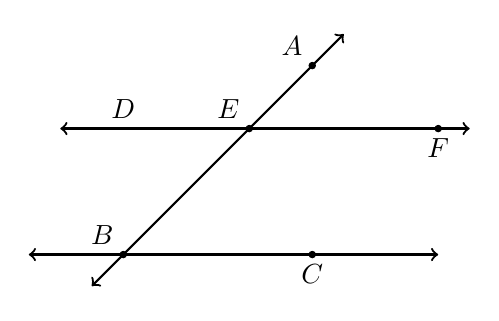
\begin{tikzpicture}[scale=0.8]
      \draw [<->, thick] (-1.5,0)--(0,0)--(5,0);
      \draw [<->, thick] (-0.5,-0.5)--(3,3)--(3.5,3.5);
      \draw [<->, thick] (-1,2)--(0,2) node [above]{$D$}--(5, 2)--(5.5,2);
      \draw [fill] (3,3) circle [radius=0.05] node[above left]{$A$};
      \draw [fill] (5, 2) circle [radius=0.05] node[below]{$F$};
      \draw [fill] (2,2) circle [radius=0.05] node[above left]{$E$};
      \draw [fill] (0,0) circle [radius=0.05] node[above left]{$B$};
      \draw [fill] (3,0) circle [radius=0.05] node[below]{$C$};
    \end{tikzpicture}

  \item Given the situation in the diagram, answer each question. Circle True or False. %\vspace{1cm}
      \begin{flushright}
      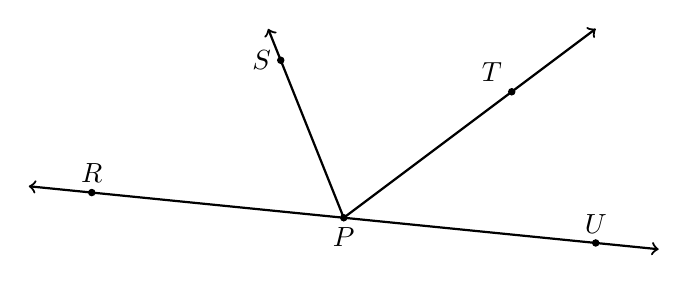
\begin{tikzpicture}[scale=0.8]
        \draw [->, thick] (0,0)--(4,3);
        \draw [<->, thick] (-5,.5)--(5,-.5);
        \draw [->, thick] (0,0)--(-1.2,3);
        \draw [fill] (-1,2.5) circle [radius=0.05] node[left ]{$S$};
        \draw [fill] (2.66666,2) circle [radius=0.05] node[above left ]{$T$};
        \draw [fill] (0,0) circle [radius=0.05] node[below]{$P$};
        \draw [fill] (4,-0.4) circle [radius=0.05] node[above]{$U$};
        \draw [fill] (-4,0.4) circle [radius=0.05] node[above]{$R$};
      \end{tikzpicture}
      \end{flushright}
    \begin{enumerate}
      \item True or False: $\angle SPU$ is an acute angle.
      \item True or False: $\overrightarrow{RP}$ and $\overrightarrow{PU}$ are opposite rays.
      \item True or False: $\angle RPS$ and $\angle SPU$ are a linear pair.
      \item True or False: $\angle SPT$ and $\angle TPR$ are adjacent.
    \end{enumerate}

 \item Find the volume of a hemisphere with a radius of three inches, to the \emph{nearest whole cubic inch}. (The formula for the volume of a \emph{sphere} is $V=\frac{4}{3}\pi r^3$)

\end{enumerate}
\newpage
\subsubsection*{Classwork: Circle the appropriate equation and state the justification}
   Use the postulates and theorems you have learned. You may abbreviate them as follows: ``def. of bisector," ``$\perp$ rays meet at $90^\circ$," ``complementary $\angle$s add to 90," ``linear pairs add to 180," ``vertical $\angle$s are $\cong$," ``corresponding $\angle$s of parallel lines are $\cong$."

\begin{enumerate}
   \item Given corresponding angles of a transversal and two parallel lines, $\angle A$, $\angle B$.\\[0.75cm]
   $\angle A \cong \angle B$ \hspace{1cm} $m \angle A + m \angle B=180^\circ$ \hspace{0.5cm} \rule{5cm}{0.15mm} \vspace{0.5cm}

   \item $\angle RPS \cong \angle SPU$ \hspace{0.25cm} $m \angle RPS + m \angle SPU = 180^\circ$ \hspace{0.25cm} \rule{6cm}{0.15mm} \\ \vspace{0.5cm}
       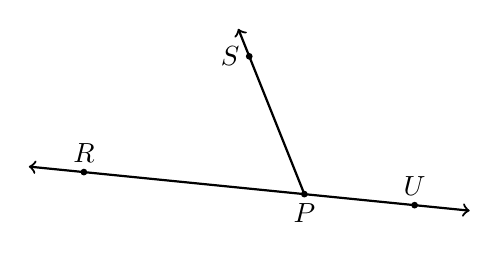
\begin{tikzpicture}[scale=0.7]
         \draw [<->, thick] (-5,.5)--(3,-.3);
         \draw [->, thick] (0,0)--(-1.2,3);
         \draw [fill] (-1,2.5) circle [radius=0.05] node[left ]{$S$};
         \draw [fill] (0,0) circle [radius=0.05] node[below]{$P$};
         \draw [fill] (2,-0.2) circle [radius=0.05] node[above]{$U$};
         \draw [fill] (-4,0.4) circle [radius=0.05] node[above]{$R$};
       \end{tikzpicture}

   \item Given $m \angle 1 = 4x+6$, $m \angle 2 = 6x-32$. Find $m \angle 1$.
       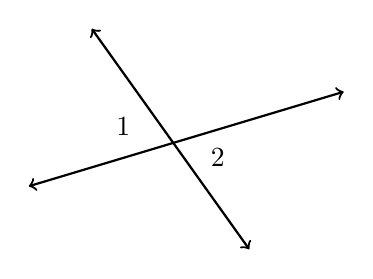
\begin{tikzpicture}[scale=.4]
         \draw [<->, thick] (0,-1.5)--(10,1.5);
         \draw [<->, thick] (2,3.5)--(7,-3.5);
         \node at (3,.4){1};
         \node at (6,-.6){2};
       \end{tikzpicture}\\[0.5cm]
       $\angle 1 \cong \angle 2$ \hspace{1cm} $m\angle 1 + m\angle 2 =  180$ \hspace{0.5cm} \rule{6cm}{0.15mm} \vspace{0.5cm}

   \item Given $m\angle R=m\angle U =65$, and $m\angle UST=130$. Find $m\angle RSU$.
   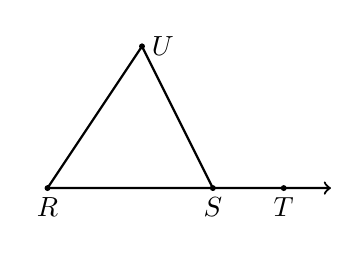
\begin{tikzpicture}[scale=0.6]
     %\draw [->, thick] (0,0)--(5,5);
     \draw [<-, thick] (7,0)--(1,0)--(3,3)--(4.5,0);
     \draw [fill] (1,0) circle [radius=0.05] node[below]{$R$};
     \draw [fill] (4.5,0) circle [radius=0.05] node[below]{$S$};
     \draw [fill] (3,3) circle [radius=0.05] node[right]{$U$};
     \draw [fill] (6,0) circle [radius=0.05] node[below]{$T$};
   \end{tikzpicture}\\[0.5cm]
   $\angle UST \cong \angle RSU$ \hspace{0.5cm} $m\angle UST + m\angle RSU =  180$ \hspace{0.5cm} \rule{6cm}{0.15mm} \vspace{1cm}

   \item Given $\overrightarrow{BA} \perp \overrightarrow{BC}$, $m \angle ABD = 2x-5$, and $m \angle DBC = x-10$.
     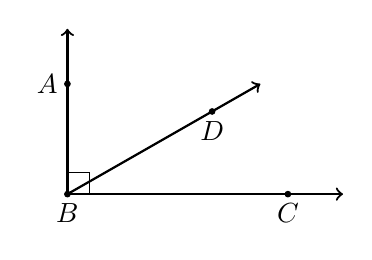
\begin{tikzpicture}[scale=0.7]
       \draw [<->, thick] (0,3)--(0,0)--(5,0);
       \draw [->, thick] (0,0)--(3.5, 2);
       \draw [-, thin] (0, 0.4)--(0.4, 0.4)--(0.4, 0);
       \draw [fill] (0,0) circle [radius=0.05] node[below]{$B$};
       \draw [fill] (0,2) circle [radius=0.05] node[left]{$A$};
       \draw [fill] (4,0) circle [radius=0.05] node[below]{$C$};
       \draw [fill] (2.625, 1.5) circle [radius=0.05] node[below]{$D$};
     \end{tikzpicture}\\[0.5cm]
     $\angle ABD \cong \angle DBC$ \hspace{0.5cm} $m\angle ABD + m\angle DBC =  90$ \hspace{0.5cm} \rule{6cm}{0.15mm}

\end{enumerate}

\end{document}
